%% Copernicus Publications Manuscript Preparation Template for LaTeX Submissions
%% ---------------------------------
%% This template should be used for copernicus.cls
%% The class file and some style files are bundled in the Copernicus Latex Package, which can be downloaded from the different journal webpages.
%% For further assistance please contact Copernicus Publications at: production@copernicus.org
%% https://publications.copernicus.org/for_authors/manuscript_preparation.html


%% Please use the following documentclass and journal abbreviations for preprints and final revised papers.

%% 2-column papers and preprints
\documentclass[hess, manuscript]{copernicus}



%% Journal abbreviations (please use the same for preprints and final revised papers)


% Advances in Geosciences (adgeo)
% Advances in Radio Science (ars)
% Advances in Science and Research (asr)
% Advances in Statistical Climatology, Meteorology and Oceanography (ascmo)
% Annales Geophysicae (angeo)
% Archives Animal Breeding (aab)
% ASTRA Proceedings (ap)
% Atmospheric Chemistry and Physics (acp)
% Atmospheric Measurement Techniques (amt)
% Biogeosciences (bg)
% Climate of the Past (cp)
% DEUQUA Special Publications (deuquasp)
% Drinking Water Engineering and Science (dwes)
% Earth Surface Dynamics (esurf)
% Earth System Dynamics (esd)
% Earth System Science Data (essd)
% E&G Quaternary Science Journal (egqsj)
% European Journal of Mineralogy (ejm)
% Fossil Record (fr)
% Geochronology (gchron)
% Geographica Helvetica (gh)
% Geoscience Communication (gc)
% Geoscientific Instrumentation, Methods and Data Systems (gi)
% Geoscientific Model Development (gmd)
% History of Geo- and Space Sciences (hgss)
% Hydrology and Earth System Sciences (hess)
% Journal of Bone and Joint Infection (jbji)
% Journal of Micropalaeontology (jm)
% Journal of Sensors and Sensor Systems (jsss)
% Magnetic Resonance (mr)
% Mechanical Sciences (ms)
% Natural Hazards and Earth System Sciences (nhess)
% Nonlinear Processes in Geophysics (npg)
% Ocean Science (os)
% Primate Biology (pb)
% Proceedings of the International Association of Hydrological Sciences (piahs)
% Scientific Drilling (sd)
% SOIL (soil)
% Solid Earth (se)
% The Cryosphere (tc)
% Weather and Climate Dynamics (wcd)
% Web Ecology (we)
% Wind Energy Science (wes)


%% \usepackage commands included in the copernicus.cls:
%\usepackage[german, english]{babel}
%\usepackage{tabularx}
%\usepackage{cancel}
%\usepackage{multirow}
%\usepackage{supertabular}
%\usepackage{algorithmic}
%\usepackage{algorithm}
%\usepackage{amsthm}
%\usepackage{float}
%\usepackage{subfig}
%\usepackage{rotating}


\begin{document}

\title{Downscaling climate timeseries in data sparse regions}


% \Author[affil]{given_name}{surname}

\Author[]{}{}
\Author[]{}{}
\Author[]{}{}

\affil[]{ADDRESS}
\affil[]{ADDRESS}

%% The [] brackets identify the author with the corresponding affiliation. 1, 2, 3, etc. should be inserted.

%% If an author is deceased, please mark the respective author name(s) with a dagger, e.g. "\Author[2,$\dag$]{Anton}{Aman}", and add a further "\affil[$\dag$]{deceased, 1 July 2019}".

%% If authors contributed equally, please mark the respective author names with an asterisk, e.g. "\Author[2,*]{Anton}{Aman}" and "\Author[3,*]{Bradley}{Bman}" and add a further affiliation: "\affil[*]{These authors contributed equally to this work.}".


\correspondence{NAME (EMAIL)}

\runningtitle{TEXT}

\runningauthor{TEXT}





\received{}
\pubdiscuss{} %% only important for two-stage journals
\revised{}
\accepted{}
\published{}

%% These dates will be inserted by Copernicus Publications during the typesetting process.


\firstpage{1}

\maketitle



\begin{abstract}
TEXT
\end{abstract}


\copyrightstatement{TEXT}


\introduction  %% \introduction[modified heading if necessary]
Climate timeseries are required at higher resolutions than currently available from GCM or even RCMs for meaningful impact studies. This is especially the case in heterogeneous terrain such as mountain regions where surface variability is high over short horizontal distances. Various methods of downscaling can be utilised to achieve this goal. Dynamical doewnscaling requires no additional data beyond boundary forcing yet is costly and generally applied to limited domains. Statistical downscaling is cheap to run yet requires extensive and robust ground data.

Here we propose a hybrid method that use the quasi-physical topography based method TopoSCALE to generate point forcing timeseries for current period then employs quantile mapping to statistically downscale or debias a climate timeseries at this point. We demonstrate this approach by downscaling CORDEX RCM data at both point scale and additionally generalising this to a spatial product using the tool TopoSUB.

This method provides full forcing suite required to run a numerical model and we further demo this for the case of snowcover in switzerland

plots

1. domain
2. basic method poit
3. method spatial
4. plot snow

\section{references}
Bias Correction of GCM Precipitation by Quantile Mapping: How Well Do Methods Preserve Changes in Quantiles and Extremes? 
Alex J. Cannon; Stephen R. Sobie; Trevor Q. Murdock
J. Climate (2015) 28 (17): 6938–6959.
https://doi.org/10.1175/JCLI-D-14-00754.1
Article history

\section{Data}





\subsection{Cordex EUR22 Regional Climate Model data}
We use data from region X EUR22 at nominal resolution of 22~km.

Should use 44km or 11km as more models available

API request 22:
%https://esgf-data.dkrz.de/esg-search/wget?project=CORDEX&variable=tas&variable=pr&time_frequency=day&domain=EUR-22&experiment=rcp26&experiment=rcp85&experiment=historical&download_structure=project,product,domain,institute,driving_model,experiment,ensemble,rcm_name,rcm_version,time_frequency,variable

API request 44:
%https://esgf-data.dkrz.de/esg-search/wget?project=CORDEX&variable=tas&variable=pr&time_frequency=day&time_frequency=3h&domain=EUR-44&experiment=rcp26&experiment=rcp85&experiment=historical&download_structure=project,product,domain,institute,driving_model,experiment,ensemble,rcm_name,rcm_version,time_frequency,variable

%https://esg-dn1.nsc.liu.se/esg-search/wget?project=CORDEX&variable=tas&variable=pr&time_frequency=day&time_frequency=3hr&domain=EUR-44&experiment=rcp26&experiment=rcp85&experiment=historical&download_structure=project,product,domain,institute,driving_model,experiment,ensemble,rcm_name,rcm_version,time_frequency,variable

%3H data download
%DONE:
%joel@mountainsense:~/sim/qmap$ ./wget-hist_TASPR.sh -H  = 41GB

%TODO
%joel@mountainsense:~/sim/qmap$ ./wget-rcp26_TASPR.sh -H
%joel@mountainsense:~/sim/qmap$ ./wget-rcp85_TAS.sh -H
%joel@mountainsense:~/sim/qmap$ ./wget-rcp85_PR.sh -H

yields 276 files (~50gb)

Historical period: 1970-2005

Data description at CDS:
https://cds.climate.copernicus.eu/portfolio/dataset/projections-cordex-single-levels

\subsection{Preprocessing}
All prercessing such as concatenating netcdf timeseries, extracting region of interest and regridding from rotated pole was done using the CDO operators
\subsection{Scripts and technical issues}

%https://github.com/joelfiddes/topoCLIM

- Calenders: 360\_day propelectic\_gregorian
- Time range: 2099-2100

\subsection{Data management strategy}

\subsection{Parameters}
%https://is-enes-data.github.io/CORDEX_variables_requirement_table.pdf
Surface Air Pressure (644)
 Surface Downwelling Longwave Radiation (1688)
 Surface Downwelling Shortwave Radiation (1726)
 





\section{Methods}

\subsection{Extreme value analysis}
%https://www.meteoswiss.admin.ch/content/dam/meteoswiss/en/service-und-publikationen/publikationen/doc/nidex_technical_report_20171018.pdf
\subsection{Intervariabele consistency after qmap}
\subsection{Downscaling current climate}


\subsection{Quantile mapping (QMAP)}

\subsection{Quantile mapping seasonal(QMAP)}
While quantile mapping ensures that quantile biases are corrected in the CDF it does not account for temporally varying bias. It is therefore well suited to TAS where we can be reasonablly sure that winters are cold and summers hot, at least in mid to high latitudes. However with precipitation interannual distribution can be biased while the cdf may look good. We address this with a two step approach called QMAP\_SEASON. We split the date according to some temporal subset, in this case "summer" (April-September) and "winter" (October - March) and run QMAP on each subset so computing to sets of QMAP parameters. These are applied throughout the historcal and climate timeseries at the approprite months

\subsection{Generalising to subdaily variables}

\subsection{Spatialisation}
\subsection{Evaluation metrics}

Statistical transformations, as any statistical technique,
quietly assume that the modelled relation holds if confronted
with new data. In the context of climate impact assessment
this assumption is critical as it has to be expected that climate variables exceed the observed range in future periods.
Further, highly adaptable methods, such as the nonparametric techniques used in this study, are prone to over fitting the
data. Both issues require that model error is quantified using
data that have not been used for calibration. A standard technique for this task is cross-validation (CV) (e.g. Hastie et al.,
2001) which has been previously applied for evaluating statistical downscaling techniques (e.g. Themeßl et al., 2011,
2012). Here a 10-fold CV was employed to produce unbiased estimates of MAE and MAE0.1, MAE0.2, ..., MAE1.0.
First the data are split into 10 subsamples of continuous time
intervals. The model is then calibrated using the data with
one of the subsamples being removed. MAE and MAE0.1,
MAE0.2, ..., MAE1.0 are then estimated using the subsample
that was not used for calibration. This procedure is repeated
for each subsample and results in 10 estimates of model error. The mean of these 10 error estimates, the so called mean
cross-validation error, is reported. In the remainder of this article MAE and MAE0.1, MAE0.2, ..., MAE1.0 always refers
to the mean cross-validation error to ease formulation.

https://link.springer.com/article/10.1007%2Fs00477-019-01750-7:
Evaluation of RQM
Practical considerations
For the evaluation of the transfer functions of both BCMs (i.e., QDM and RQM), we split the data into two periods; one for calibration and the other for validation, which is an approach widely applied in bias correction (Michelangeli et al. 2009; Piani et al. 2010a, b; Hempel et al. 2013; Vrac and Friederichs 2015). Here, the calibration period (CP) covers the years from 1960 to 1982, while the validation period (VP) includes the years from 1983 to 2005. Hence, each period covers 23 years of observed and modeled data. Note that the performed splitting implicitly assumes that all distributional changes in both observed and modeled data are the same during both periods, which should in general be critically assessed since trends may be nonlinear or just cannot be disentangled from low frequency variability. Nonetheless, making this assumption is crucial to be able to perform a detailed evaluation of the two BCMs’ respective performance characteristics.

The CP is used to calibrate both, QDM 
\section{Results}



\conclusions  %% \conclusions[modified heading if necessary]
TEXT

%% The following commands are for the statements about the availability of data sets and/or software code corresponding to the manuscript.
%% It is strongly recommended to make use of these sections in case data sets and/or software code have been part of your research the article is based on.

\codeavailability{TEXT} %% use this section when having only software code available


\dataavailability{TEXT} %% use this section when having only data sets available


\codedataavailability{TEXT} %% use this section when having data sets and software code available


\sampleavailability{TEXT} %% use this section when having geoscientific samples available


\videosupplement{TEXT} %% use this section when having video supplements available


\appendix
\section{}    %% Appendix A

\subsection{}     %% Appendix A1, A2, etc.


\noappendix       %% use this to mark the end of the appendix section. Otherwise the figures might be numbered incorrectly (e.g. 10 instead of 1).

%% Regarding figures and tables in appendices, the following two options are possible depending on your general handling of figures and tables in the manuscript environment:

%% Option 1: If you sorted all figures and tables into the sections of the text, please also sort the appendix figures and appendix tables into the respective appendix sections.
%% They will be correctly named automatically.

%% Option 2: If you put all figures after the reference list, please insert appendix tables and figures after the normal tables and figures.
%% To rename them correctly to A1, A2, etc., please add the following commands in front of them:

\appendixfigures  %% needs to be added in front of appendix figures

\appendixtables   %% needs to be added in front of appendix tables

%% Please add \clearpage between each table and/or figure. Further guidelines on figures and tables can be found below.



\authorcontribution{TEXT} %% this section is mandatory

\competinginterests{TEXT} %% this section is mandatory even if you declare that no competing interests are present

\disclaimer{TEXT} %% optional section

\begin{acknowledgements}
TEXT
\end{acknowledgements}




%% REFERENCES

%% The reference list is compiled as follows:

\begin{thebibliography}{}

\bibitem[AUTHOR(YEAR)]{LABEL1}
REFERENCE 1

\bibitem[AUTHOR(YEAR)]{LABEL2}
REFERENCE 2

\end{thebibliography}

%% Since the Copernicus LaTeX package includes the BibTeX style file copernicus.bst,
%% authors experienced with BibTeX only have to include the following two lines:
%%
%% \bibliographystyle{copernicus}
%% \bibliography{example.bib}
%%
%% URLs and DOIs can be entered in your BibTeX file as:
%%
%% URL = {http://www.xyz.org/~jones/idx_g.htm}
%% DOI = {10.5194/xyz}


%% LITERATURE CITATIONS
%%
%% command                        & example result
%% \citet{jones90}|               & Jones et al. (1990)
%% \citep{jones90}|               & (Jones et al., 1990)
%% \citep{jones90,jones93}|       & (Jones et al., 1990, 1993)
%% \citep[p.~32]{jones90}|        & (Jones et al., 1990, p.~32)
%% \citep[e.g.,][]{jones90}|      & (e.g., Jones et al., 1990)
%% \citep[e.g.,][p.~32]{jones90}| & (e.g., Jones et al., 1990, p.~32)
%% \citeauthor{jones90}|          & Jones et al.
%% \citeyear{jones90}|            & 1990



%% FIGURES

%% When figures and tables are placed at the end of the MS (article in one-column style), please add \clearpage
%% between bibliography and first table and/or figure as well as between each table and/or figure.

% The figure files should be labelled correctly with Arabic numerals (e.g. fig01.jpg, fig02.png).


%% ONE-COLUMN FIGURES

%%f
%\begin{figure}[t]
%\includegraphics[width=8.3cm]{FILE NAME}
%\caption{}
%\end{figure}
%
 \clearpage
%%% TWO-COLUMN FIGURES
%
%f
\begin{figure*}[t]
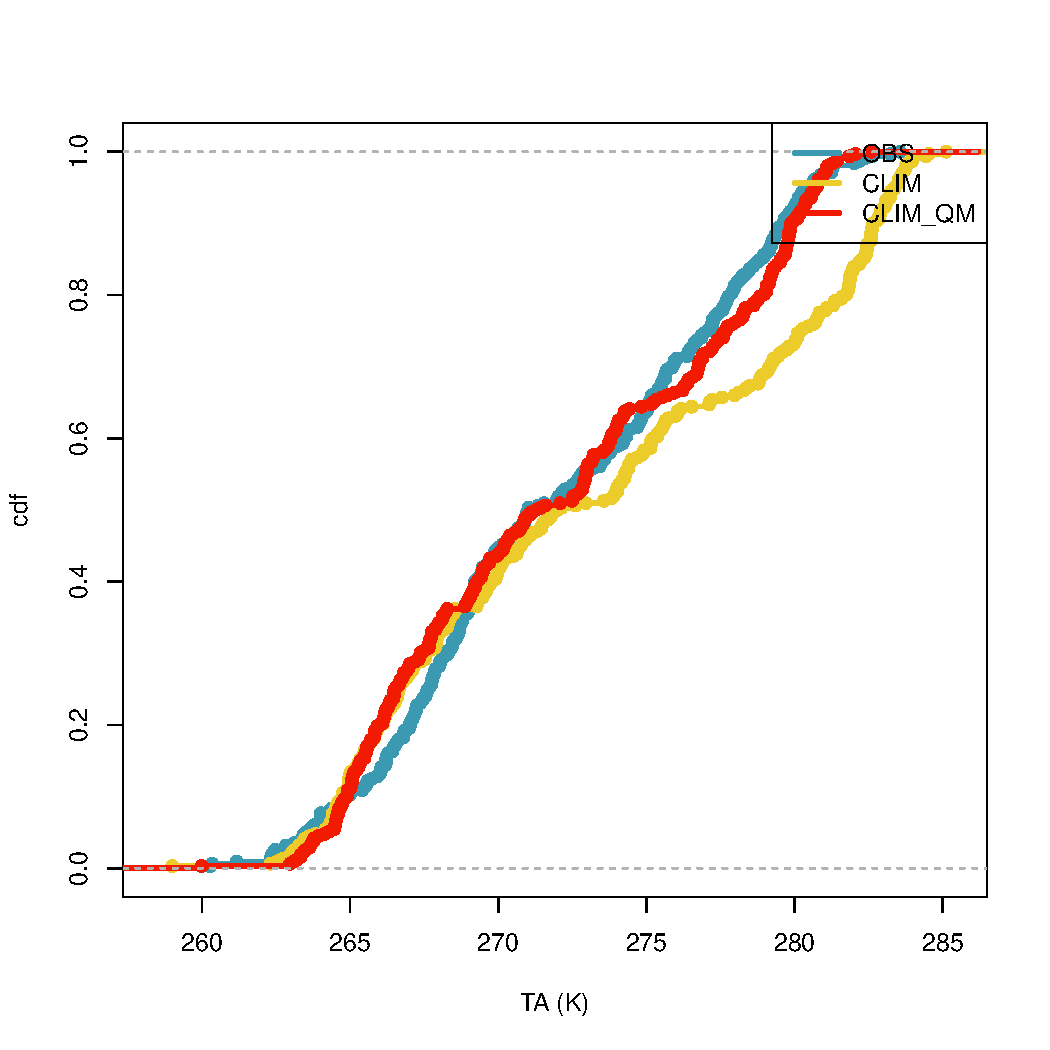
\includegraphics[width=12cm]{"plots/TA_CDF.pdf"}
\caption{ }
\end{figure*}

\begin{figure*}[t]
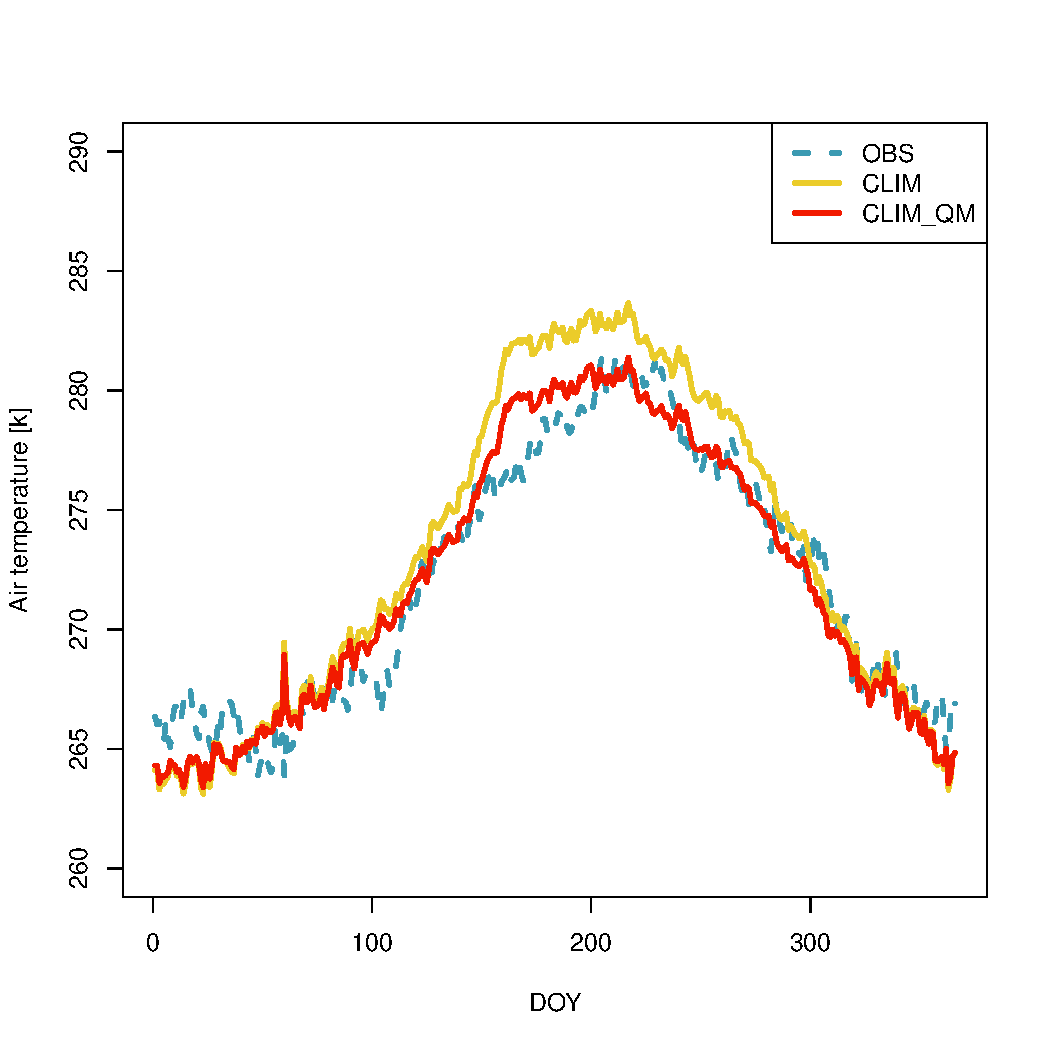
\includegraphics[width=12cm]{"plots/TA_DOY.pdf"}
\caption{}
\end{figure*}

\begin{figure*}[t]
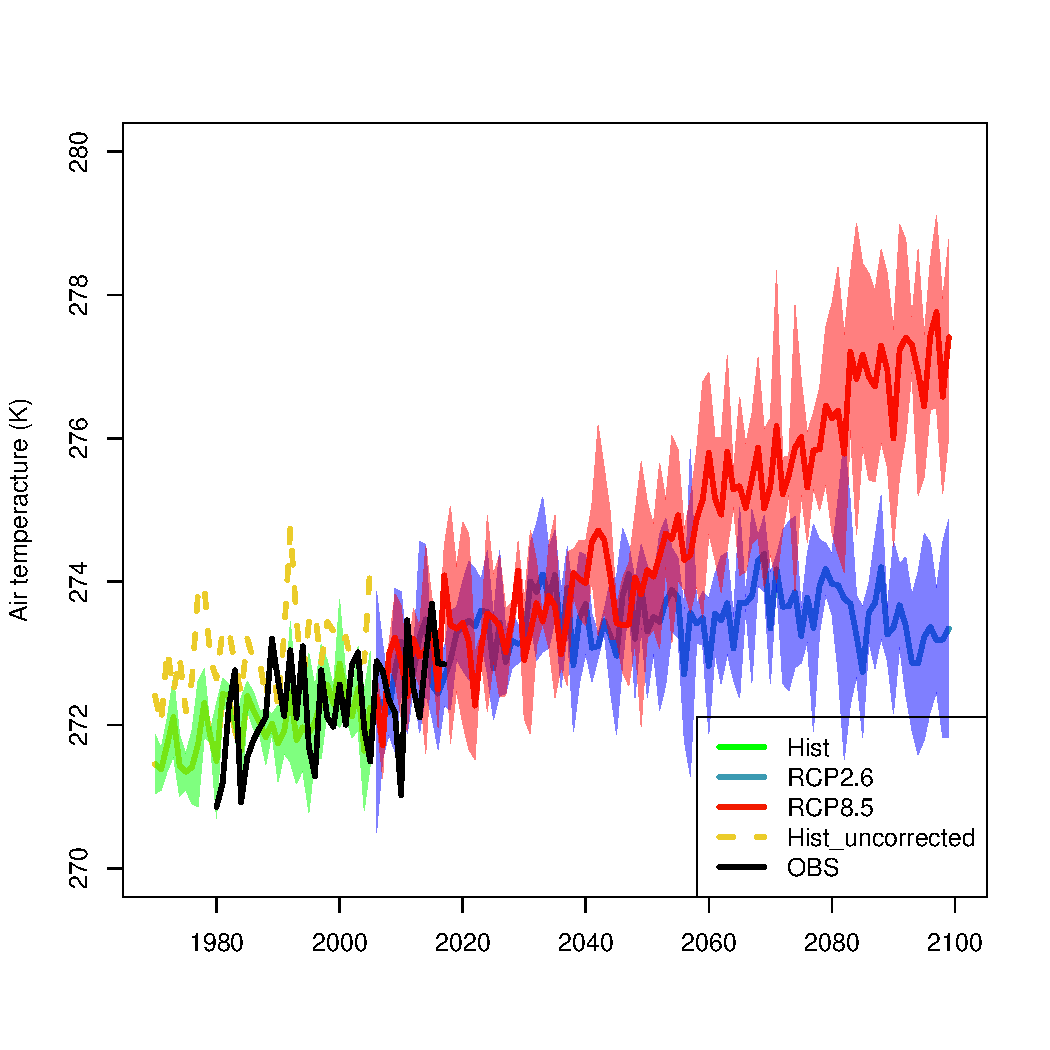
\includegraphics[width=12cm]{"plots/TA_TS.pdf"}
\caption{Mean annual near surface air temperature at the Weissfluhjoch (2540m asl)  showing corrected historical, RCP2.6 and RCP8.5 timseries. Observations and uncorrected historical data are also shown for comparison. The coloured envelops indicate +/- 1 SD of the model spread and multi-modal mean is given by the bold line. }
\end{figure*}

\begin{figure*}[t]
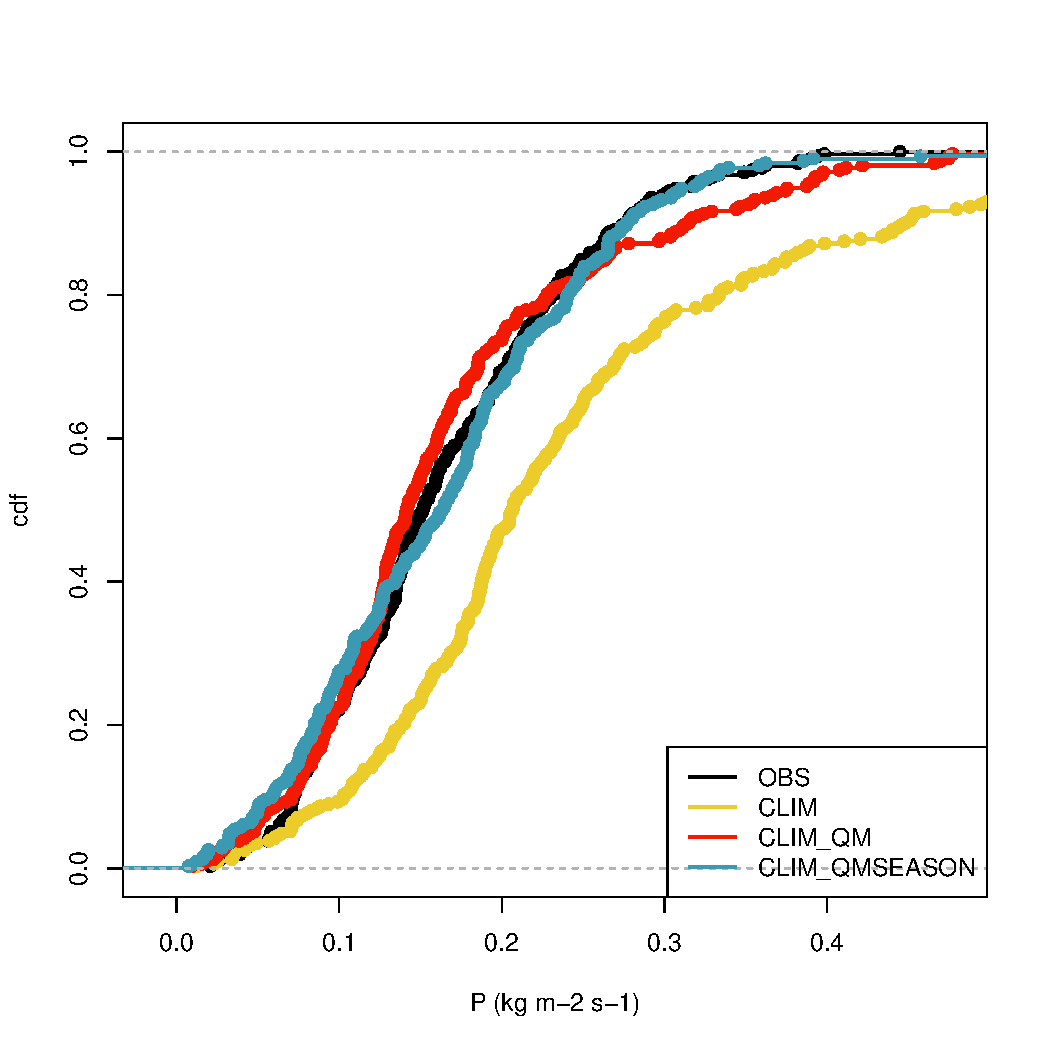
\includegraphics[width=12cm]{"plots/P_CDF.pdf"}
\caption{Multi-modal Mean monthly precipitation rate ($kg m^{-2} s^{-1}$) at the Weissfluhjoch (2540m asl) . This shows the improvements in the CDF by QMAP and further improvements (interannual distribution) with QMAP_SEASON. }
\end{figure*}

\begin{figure*}[t]
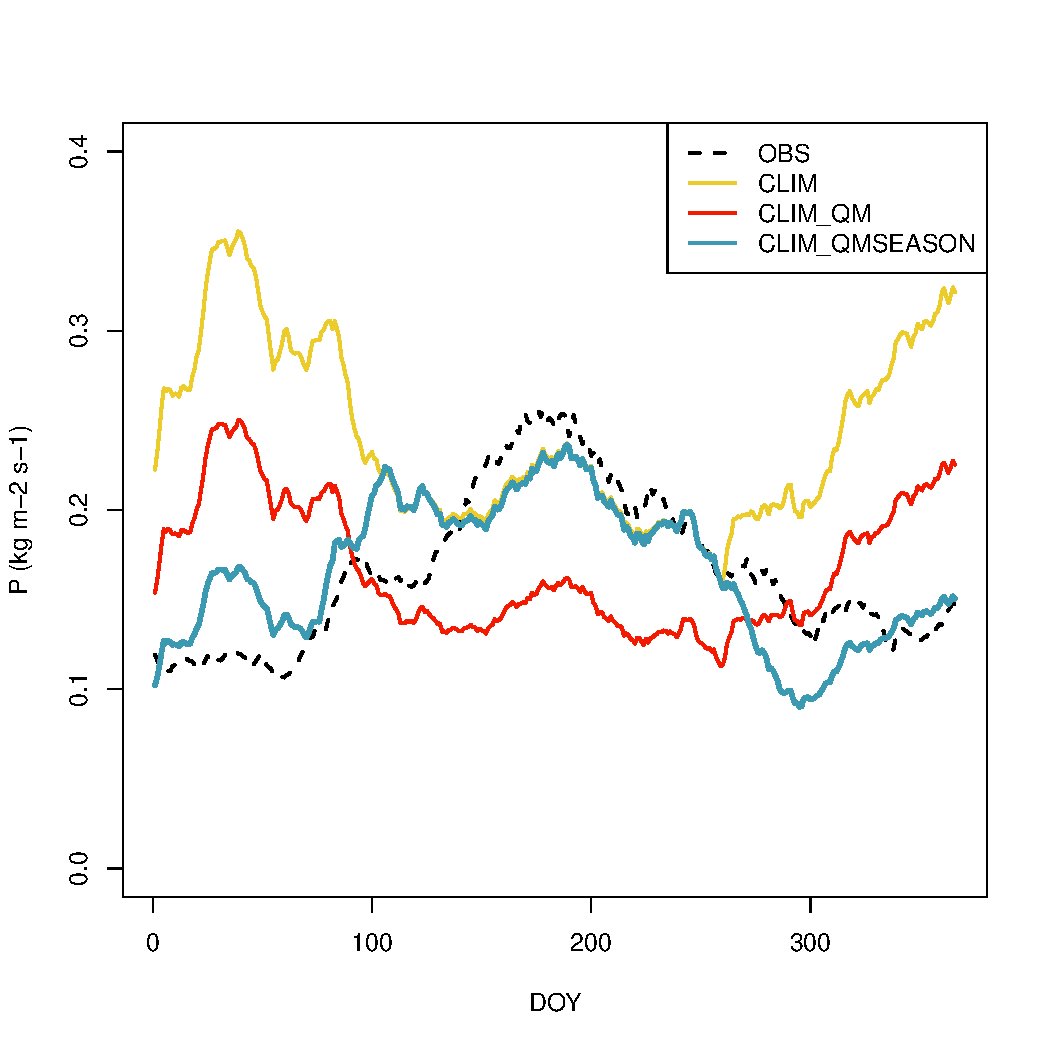
\includegraphics[width=12cm]{"plots/P_DOY.pdf"}
\caption{Multi-modal Mean daily precipitation rate ($kg m^{-2} s^{-1}$) at the Weissfluhjoch (2540m asl). This shows the improvements in the CDF by QMAP and further improvements (interannual distribution) with QMAP_SEASON. A 30-day running mean filter is applied for clarity. }
\end{figure*}

\begin{figure*}[t]
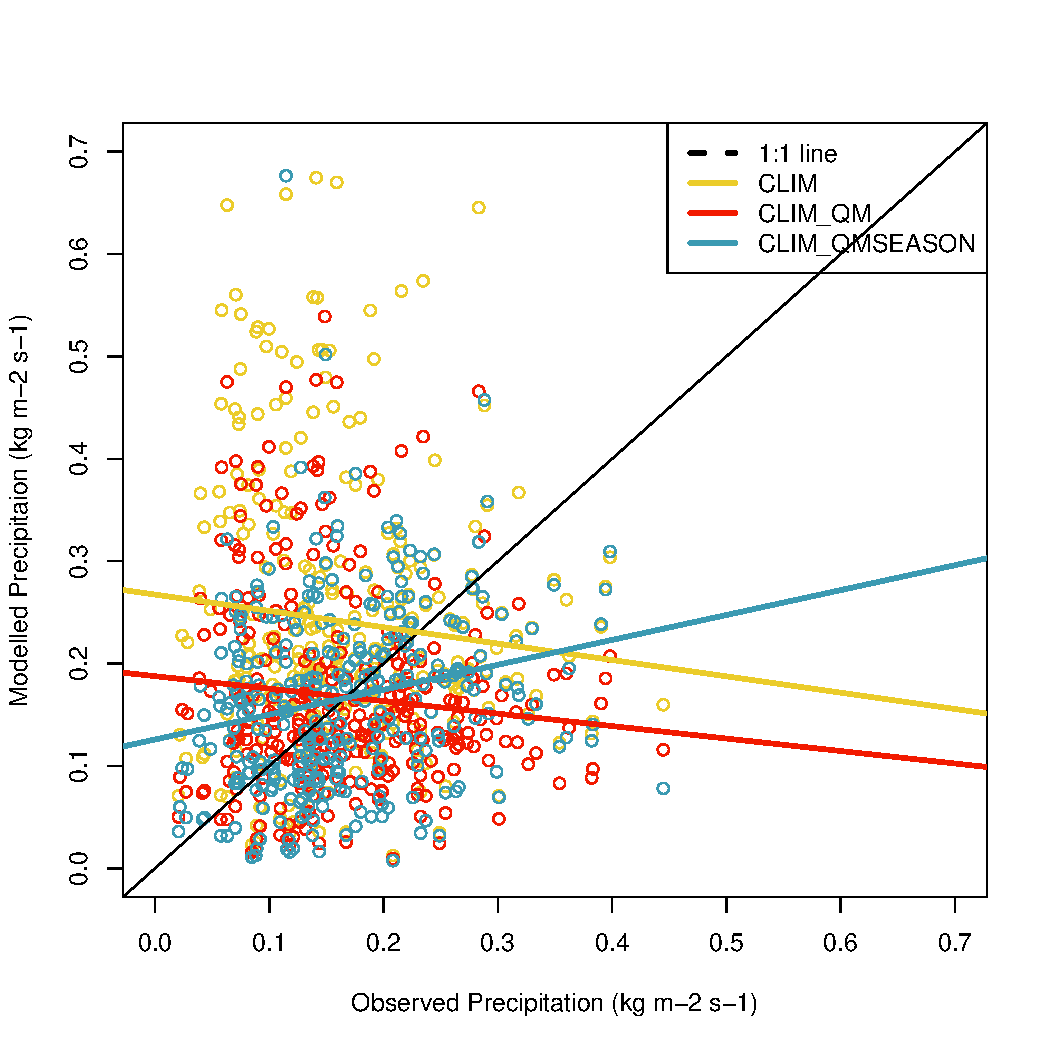
\includegraphics[width=12cm]{"plots/P_SCATTER.pdf"}
\caption{Multi-modal Mean daily precipitation rate ($kg m^{-2} s^{-1}$) at the Weissfluhjoch (2540m asl). This shows the improvements in the CDF by QMAP and further improvements (interannual distribution) with QMAP_SEASON. A 30-day running mean filter is applied for clarity. }
\end{figure*}


%
%
 \clearpage
%%% TABLES
%%%
 \begin{table}[t]
 \begin{center}
% \begin{sidewaystable*}[t]
 \caption{CORDEX variables used in this study, togther with the Climate and Forecast Conventions (CF) standard name .}
 \begin{tabular}{l l l l l }
 \hline
 output variable name  &units  & long\_name  &CF standard\_name \\
  \hline
 tas  &K  & Near-Surface Air Temperature  &air\_temperature  \\
 pr & kg m-2 s-1  &Precipitation  &precipitation\_flux \\
 ps & Pa  &Surface Air Pressure  &surface\_air\_pressure  \\
 hurs & \%    &Near-Surface Relative  &Humidity relative\_humidity \\
 rsds  &W m-2  & Surface Downwelling Shortwave Radiation & surface\_downwelling\_shortwave\_flux\_in\_air   \\
rlds  &W m-2 & Surface Downwelling Longwave Radiation & surface\_downwelling\_longwave\_flux\_in\_air\\
uas  &m s-1 &Eastward  Near-Surface Wind &eastward\_wind  \\
vas &m s-1 &Northward  Near-Surface Wind &northward\_wind \\

 \hline  
 \end{tabular}
 \label{tab:01}
% \end{sidewaystable*}
 \end{center}
\end{table}


% Table created by stargazer v.5.2.2 by Marek Hlavac, Harvard University. E-mail: hlavac at fas.harvard.edu
% Date and time: Fr, Jul 03, 2020 - 12:27:21
\begin{table}[!htbp] \centering 
  \caption{} 
  \label{} 
\begin{tabular}{@{\extracolsep{5pt}} ccccc} 
\\[-1.8ex]\hline 
\hline \\[-1.8ex] 
 & OBS & Hist & Hist\_QMAP & Hist\_QMAPSEASON \\ 
\hline \\[-1.8ex] 
MEAN & $0.170$ & $0.240$ & $0.170$ & $0.170$ \\ 
R-COR & $-$ & $$-$0.090$ & $$-$0.100$ & $0.210$ \\ 
RMSE & $-$ & $0.180$ & $0.130$ & $0.110$ \\ 
\hline \\[-1.8ex] 
\end{tabular} 
\end{table}
%%% The different columns must be seperated with a & command and should
%%% end with \\ to identify the column brake.
%
%%% ONE-COLUMN TABLE
%
%%t
%\begin{table}[t]
%\caption{TEXT}
%\begin{tabular}{column = lcr}
%\tophline
%
%\middlehline
%
%\bottomhline
%\end{tabular}
%\belowtable{} % Table Footnotes
%\end{table}
%
%%% TWO-COLUMN TABLE
%
%%t
%\begin{table*}[t]
%\caption{TEXT}
%\begin{tabular}{column = lcr}
%\tophline
%
%\middlehline
%
%\bottomhline
%\end{tabular}
%\belowtable{} % Table Footnotes
%\end{table*}
%
%%% LANDSCAPE TABLE
%
%%t
%\begin{sidewaystable*}[t]
%\caption{TEXT}
%\begin{tabular}{column = lcr}
%\tophline
%
%\middlehline
%
%\bottomhline
%\end{tabular}
%\belowtable{} % Table Footnotes
%\end{sidewaystable*}
%
%
%%% MATHEMATICAL EXPRESSIONS
%
%%% All papers typeset by Copernicus Publications follow the math typesetting regulations
%%% given by the IUPAC Green Book (IUPAC: Quantities, Units and Symbols in Physical Chemistry,
%%% 2nd Edn., Blackwell Science, available at: http://old.iupac.org/publications/books/gbook/green_book_2ed.pdf, 1993).
%%%
%%% Physical quantities/variables are typeset in italic font (t for time, T for Temperature)
%%% Indices which are not defined are typeset in italic font (x, y, z, a, b, c)
%%% Items/objects which are defined are typeset in roman font (Car A, Car B)
%%% Descriptions/specifications which are defined by itself are typeset in roman font (abs, rel, ref, tot, net, ice)
%%% Abbreviations from 2 letters are typeset in roman font (RH, LAI)
%%% Vectors are identified in bold italic font using \vec{x}
%%% Matrices are identified in bold roman font
%%% Multiplication signs are typeset using the LaTeX commands \times (for vector products, grids, and exponential notations) or \cdot
%%% The character * should not be applied as mutliplication sign
%
%
%%% EQUATIONS
%
%%% Single-row equation
%
%\begin{equation}
%
%\end{equation}
%
%%% Multiline equation
%
%\begin{align}
%& 3 + 5 = 8\\
%& 3 + 5 = 8\\
%& 3 + 5 = 8
%\end{align}
%
%
%%% MATRICES
%
%\begin{matrix}
%x & y & z\\
%x & y & z\\
%x & y & z\\
%\end{matrix}
%
%
%%% ALGORITHM
%
%\begin{algorithm}
%\caption{...}
%\label{a1}
%\begin{algorithmic}
%...
%\end{algorithmic}
%\end{algorithm}
%
%
%%% CHEMICAL FORMULAS AND REACTIONS
%
%%% For formulas embedded in the text, please use \chem{}
%
%%% The reaction environment creates labels including the letter R, i.e. (R1), (R2), etc.
%
%\begin{reaction}
%%% \rightarrow should be used for normal (one-way) chemical reactions
%%% \rightleftharpoons should be used for equilibria
%%% \leftrightarrow should be used for resonance structures
%\end{reaction}
%
%
%%% PHYSICAL UNITS
%%%
%%% Please use \unit{} and apply the exponential notation


\end{document}
